% Set up the document class for an article
\documentclass[11pt,twocolumn]{article}

% This packages permits using $ \therefore $
\usepackage{amssymb}
\usepackage{graphicx}

% This package allows the use of $ \text{} $
\usepackage{amsmath}

% The document title and author
\title{Fortune Cookie\\Datasheet Summary}
\author{Imported China Tech, LLC}

% Begin the document
\begin{document}
    \maketitle
  
    \begin{figure}
    \centering
    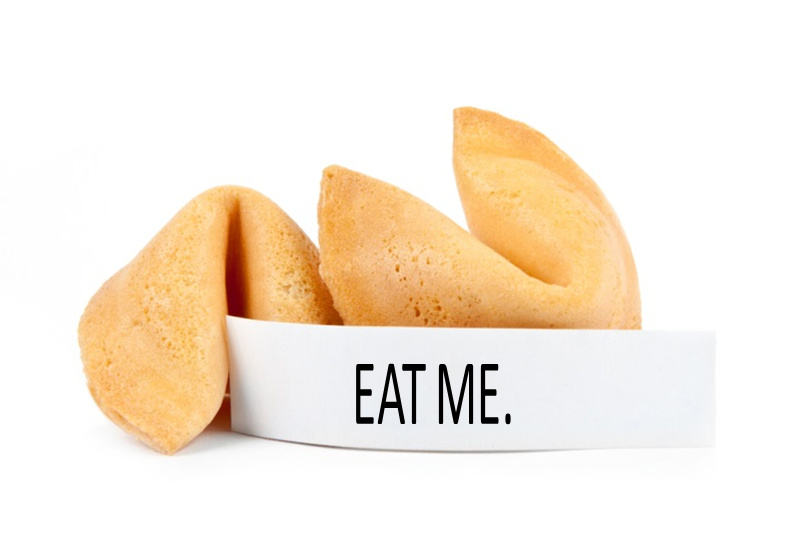
\includegraphics[height=5cm]{cookie.png}
    \caption{Professionally photographed ridiculously photogenic cookie and demo display.}
    \label{fig:la}
    \end{figure}

\section{Specification}
    \begin{itemize}
        \item Built-in retina resolution thermal printer with LPT interface
        \item SAI audio codec
        \item Two pushbuttons (user and reset)
        \item 128-Mbit Quad-SPI Flash memory
        \item 128-Mbit SDRAM (64 Mbits accessible)
        \item USB OTG HS with Micro-AB connectors
        \item Ethernet connector compliant with IEEE-802.3-2002
    \end{itemize}

\section{Usage}
\subsection{Thermal Printer Interface}
    This fortune cookie model supports the standard LPT printing interface from the last century. The user can find low cost surplus parts in many retail environments. High speed mode supports 0.4 letters per second whereas standard mode is 0.15 letters per second. Plug in the LPT cable, fight with the receipt tape loader, and crack open the cookie to produce output. Quotes are pulled from the standard Department of Engrish and Confusion Sayings API.

    \begin{figure}
    \centering
    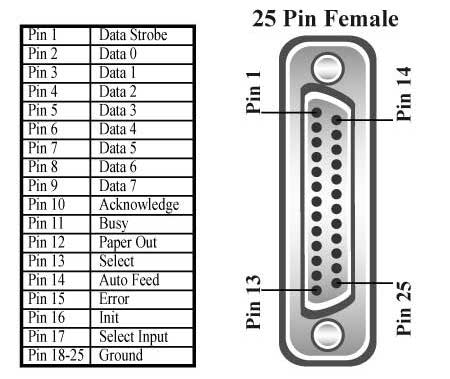
\includegraphics[height=5cm]{lptport.jpg}
    \caption{Standard LPT connector from the 1990s}
    \label{fig:lptport}
    \end{figure}
  
\end{document}